
%----------------------------------------------------------------------------------------
%	Lecture 18
%----------------------------------------------------------------------------------------

\chapter{Green's Theorem}

\bigbreak

Let's say we want to calculate the line integral over a closed curve of a vector field.
We can calculate via the definition or we can use green's theorem.

\begin{mdframed}
\begin{center}
{\bf Green's Theorem : } If $C$ is a closed curve, enclosing a region $R$, $C$ goes counterclockwise 
and vector field {\bf F} is defined and differentiable in $R$ then
$$
\oint_C {\bf F} \cdot d{\bf r} = \iint_R curl({\bf F}) dA
$$
OR
$$
\oint_C Mdx + Ndy = \iint_R (N_x - M_y) dA
$$
\end{center}
\end{mdframed}

\section{Special Case : $curl({\bf F}) = 0$ }

Since, $curl({\bf F}) = 0$ then $$\oint_C {\bf F} \cdot d{\bf r} = \iint_R curl({\bf F}) dA = 0$$

{\bf Consequence} : If {\bf F} is defined everywhere in the plane and $curl({\bf F}) = 0$ then {\bf F} is conservative.

\section{Proof of Green's Theorem}

\subsection{Finding Line Integral Over A Infinitesimal Area}

Let us take a small area $dA$ with sides $dx$ and $dy$ so $dA = dx dy$ at a point $A = (x, y)$.

\begin{figure}[ht!]
    \centering
    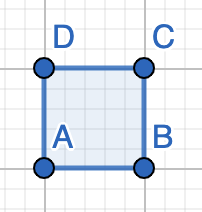
\includegraphics[scale=0.8]{./images/lecture_18_figure_1.png}
    \caption{The area element $dA$}
\end{figure}

Let our curve go along the direction $A \to B \to C \to D \to A$ such that $AB = CD = dx$ and $BC = AD = dy$.
So our line integral becomes,
\begin{align*}
\int_{ABCDA} M(x, y)dx + N(x, y)dy & = \int_{AB} M(x, y) dx + \int_{BC} N(x+dx, y) dy  \\
& \quad + \int_{CD} M(x+dx, y+dy) dx + \int_{DA} N(x, y+dy) dy \\
\\
\oint_{ABCDA} M(x, y)dx + N(x, y)dy & = M(x, y) dx + N(x + dx, y) dy - M(x+dx, y+dy) dx - N(x, y+dy) dy \\
\end{align*}

Now, 
\begin{align*}
M(x + dx, y + dy) & = M(x, y) + M_x(x, y) dx + M_y(x, y) dy \\
N(x + dx, y) & = N(x, y) + N_x(x, y) dx \\
N(x, y + dy) & = N(x, y) + N_y(x, y) dy \\
\end{align*}

Substituting these in the above, we get
\begin{align*}
\oint_{ABCDA} M(x, y) dx + N(x, y) dy & = M(x, y) dx + N(x, y) dy + N_x(x, y) dx dy \\
& - M(x, y) dx - M_x(x, y) (dx)^2 - M_y(x, y) dy dx \\
& - N(x, y) dy - N_y(x, y) (dy)^2
\end{align*}

We can ignore the $(dx)^2$ and $(dy)^2$ terms as they tend to zero as we take the limit 
and cancel out some other terms to get,

$$
\oint_{ABCDA} M(x, y) dx + N(x, y) dy = N_x(x, y) dx dy - M_y(x, y) dx dy = curl({\bf F}) dA
$$


\subsection{Combining Line Integrals of Infinitesimal Areas}

\begin{figure}[ht!]
    \centering
    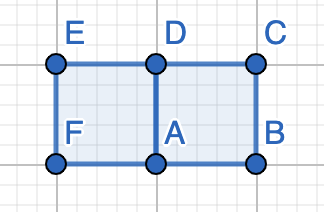
\includegraphics[scale=0.8]{./images/lecture_18_figure_2.png}
    \caption{Two curves}
\end{figure}

Let's say we want to find the line integral over $ABCDEFA$. 
We can break it up into $AB, BC, CD, DE, EF$ and $FA$.

The line integral along $ABCDA$ is sum of line integrals over $AB, BC, CD$ and $DA$.
The line integral along $ADEFA$ is sum of line integrals over $AD, DE, EF$ and $FA$.

Since we know that changing the direction of the line integral just changes the sign of the integral.
Thus, the line integral over $DA$ and $AD$ are just negatives of each other so their sum will be zero.

Now, the line integral over $ABCDEFA$ can be written as sum of line integrals over $ABCDA$ and $ADEFA$.
$$
\oint_{ABCDEFA} {\bf F} \cdot d{\bf r} = \oint_{ABCDA} {\bf F} \cdot d{\bf r}  + \oint_{ADEFA} {\bf F} \cdot {\bf r}
$$


\subsection{Conclusion}

Let's say we want to find the line integral over a closed curve $C$ which encloses a region $R$.
According to the last equation, we can break up any closed integral into line integrals over the divided region.
So let's say the we divide the region into many small rectangles of infinitesimal area $dA$. Thus, 
$$
\oint_C {\bf F} \cdot d{\bf r} = \sum_i \oint_{dA_i} {\bf F} \cdot d{\bf r}
$$

Earlier we proved that $$\oint_{dA} {\bf F} \cdot d{\bf r} = curl({\bf F}) dA $$
So using that we get,
$$
\oint_C {\bf F} \cdot d{\bf r} = \sum_i curl({\bf F}) dA_i
$$

We can calculate the above sum by using a double integral as the area $dA_i$ are infinitesimal.
Thus,
$$
\oint_C {\bf F} \cdot d{\bf r} = \iint_R curl({\bf F}) DA
$$

\section{Application}

Let's say you want to compute an integral over the circle of radius $1$ centered at $(2, 0)$ in the counterclockwise direction.
$$
\int_C ye^{-x} dx + (\frac{x^2}{2} - e^{-x}) dy
$$
Here, $M = ye^{-x}$ and $N = x^2/2 - e^{-x}$.
Thus, $curl({\bf F}) = N_x - M_y = (x^2 + e^{-x}) - e^{-x} = x$.
Thus, by green's theorem our integral becomes,
$$ \iint_R x dA = Area(R) \cdot x_{CM} $$

But we can see that this is just equal to $Area(R) \cdot x_{CM}$ where $x_{CM}$ is the $x$ coordinate of the center of mass of the region.
By symmetry, since it is a circle, its center of mass will be at its center so $x_{CM} = 2$.
And since the radius is $1$ so the area will be $\pi$.

Thus, our integral evaluates to $2\pi$.


